\chapter{Sampling, A/D and D/A Conversions}
\section{Impulse response} \label{sec:conv:impulseresponse}
	
	Linear time-invariant (LTI) systems can be fully described by the \de{impulse response} $h(\cdot)$ (both for the continuous and discrete-time case):
	\begin{equation}
		h(\cdot) = G\{ \delta(\cdot) \}
	\end{equation}
	where $y=G(x)$ is the expression that related the input $x$ of the system with it's output $y$ and $\delta$ is the pulse function. Depending  on the behaviour of the impulse response we can classify LTIs system as
	\begin{itemize}
		\item \textbf{FIR} \textit{Finite Impulse response} if there's a time $t_0$ (or $n_0$ for discrete-time systems) such that
		\[ h(t) = 0 \qquad \forall t > t_0 \]
		\item \textbf{IIR} \textit{Infinite Impulse Response} when the previous relation isn't satisfied and so the impulse response \textit{infinitely propagates}.
	\end{itemize}
	The impulse response $h(\cdot)$ is relevant because it permits to fully describe the output $y(\cdot)$ of the system to any generic input signal $x(\cdot)$ as the convolution between the two functions:
	\begin{equation} \label{eq:conv:imprestime}
		y(\cdot) = x(\cdot) * h(\cdot)
	\end{equation}
	
	\begin{proof}
		Considering a discrete-time, time-invariant linear system characterized by a transfer function $G$ and input sequence in the form
		\[ x(n) = \infsum k x(k) \delta(n-k) \]
		then the output of the system can be computed considering the linearity property of the transfer function as
		\[ y(n) = \left\{ \infsum k x(k) \delta(n-k) \right\} = \infsum k x(n) T\big\{ \delta(n-k) \big\} \]
		Having that the system is also time-invariant, then it means that the response $T\{\delta(n-k)\} = h(n-k)$ is constant and so 
		\[ y(n) = \infsum k x(k) h(n-k) = x(n) * h(n) \]	
		
		Continuous-time system can be proven instead as \textit{discretization} of the continuous time signal into a sequence of infinitesimally small rectangles:
		\[ x(t) = \lim_{\tau\rightarrow0} \infsum k x(k\tau) \rect_\tau(t-k\tau) \]	
		Considering the linearity property of the transfer function $G$ then
		\[ y(t) = \lim_{\tau\rightarrow0} G\left\{ \infsum k x(k\tau) \rect_\tau(t-k\tau) \right\} = \lim_{\tau\rightarrow0} \infsum k x(k\tau) G \left\{ \frac 1 \tau  \rect_\tau(t-k\tau) \right\} \tau \]
		Geometrically the function $\frac 1 \tau \rect_\tau(t-k\tau)$ represent a rectangle whose area is always one and having $\tau\rightarrow 0$ such function tends to the Dirac's pulse: the response $T\left\{ \frac 1 \tau \rect_\tau(t-k\tau) \right\}$ can be considered as the impulse response $h(t-k\tau)$ of the system, hence
		\[ y(t) = \lim_{\tau\rightarrow 0} \infsum k x(k\tau) h(t-k\tau)\tau = \intinf x(\tau) h(t-\tau)\, d\tau = x(t) * h(t) \]
	\end{proof}

	\paragraph{Analysis in the frequency domain}  Equation \ref{eq:conv:imprestime} relates the output of the system as the convolution between the input and the impulse response in the time domain, and so it seems naturally to analyse a system also in the frequency domain. Using the Fourier transform we can compute the \de{frequency response} $H(\cdot) = \four{h(\cdot)}$ of the linear time-invariant system; such function is characterised by a \textbf{magnitude response} $|H(\cdot)|$ and a \textbf{phase response} $\angle H(\cdot)$. \\	
	Due to having $h(\cdot)$ as a real-evaluated function, then in the frequency domain the magnitude present an even symmetry while the phase is a odd function.
	
	Considering the convolution property of the Fourier transform (eq. \ref{eq:four:convolution}, page \pageref{eq:four:convolution}) the output of the system in the frequency domain can be compute as
	\begin{equation}
		Y(\cdot) = H(\cdot) X(\cdot)
	\end{equation}
	
\section{Analog-to-digital converter}
		
		An \de{analog-to-digital converted} \textbf{ADC}, as the name says, is an electrical circuit that's used to converted an analog signal (like voltages) into digital binary data that can be elaborated by PC's. In this section high level overview of the steps to perform for this operation is presented, with particular attention to signal processing problems and related solutions that can be adopted.	
				
		\begin{figure}[bht]
			\centering
			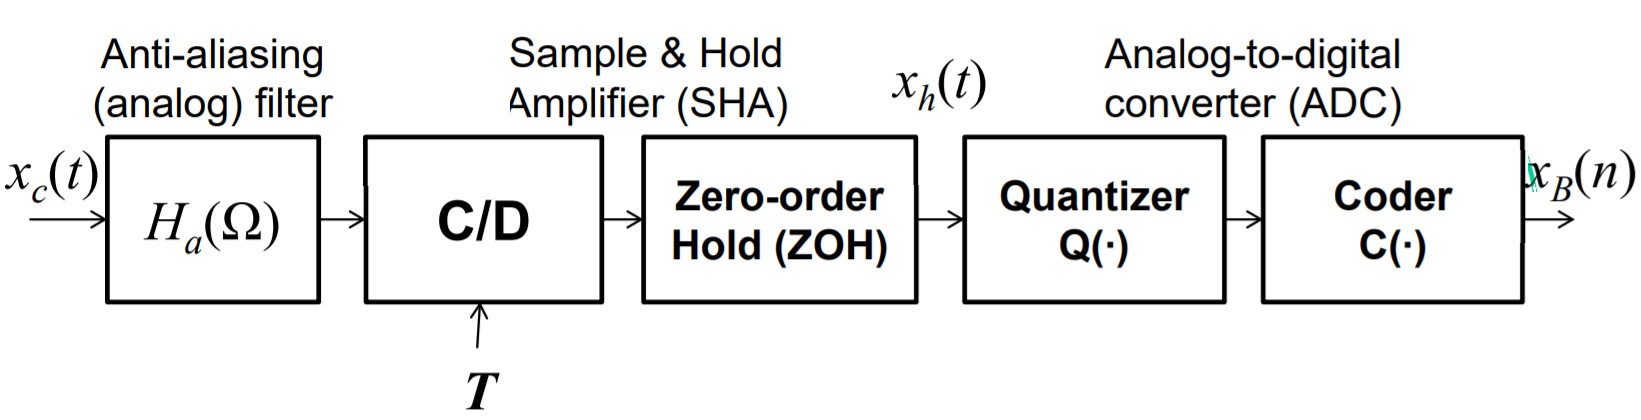
\includegraphics[width=10cm]{adc-steps}
			\caption{schematic representation of the steps used to perform an analog-to-digital conversion.} \label{fig:conv:adc}
		\end{figure}
		
		Considering the block diagram in figure \ref{fig:conv:adc}, to perform the analog-to-digital conversion the following steps are usually performed:
		\begin{enumerate}
			\item before doing the proper conversion, the analog signal is pre-processed in the analog domain by an anti-aliasing filter;
			\item with a sample\&hold amplifier the continuous time signal is discretized in the time domain (with a sampling time $T_s$) and is kept constant with a zero-order hold;
			\item the proper analog-to-digital conversion happens with the quantization (discretization in the signal domain) of the signal and it's consequence binary codification; usually this operations are performed at the same time.
		\end{enumerate}
				
		\subsection{Ideal filters} \label{sec:conv:filters}
			
			A \de{filter} is (typically) a linear system selective in the frequency domain that so determines which frequencies should be accepted and the one that should be removed.
			
			\begin{figure}[b]
				\centering 
				\begin{subfigure}{0.48\linewidth}
					\centering 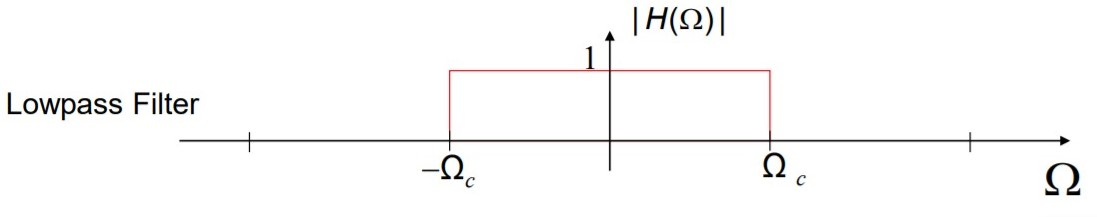
\includegraphics[width=\linewidth]{filter-low} \caption{}
				\end{subfigure} \\
				\begin{subfigure}{0.48\linewidth}
					\centering 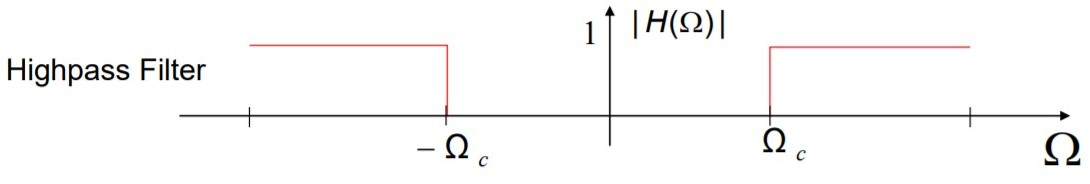
\includegraphics[width=\linewidth]{filter-high} \caption{}
				\end{subfigure}			
				\begin{subfigure}{0.48\linewidth}
					\centering 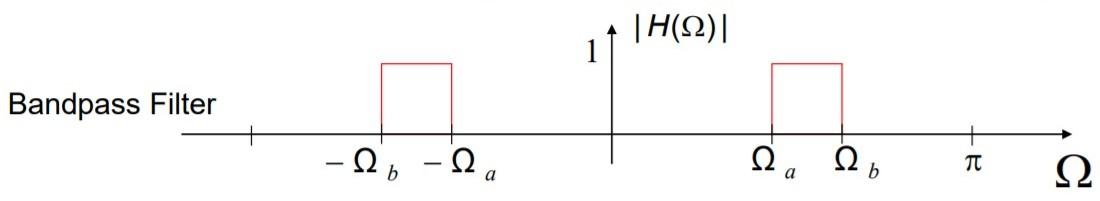
\includegraphics[width=\linewidth]{filter-band} \caption{}
				\end{subfigure}
				\caption{low-pass filter (a), high-pass filter (b) and band-pass filter (c) frequency response.} \label{fig:conv:idealfilters}
			\end{figure}
			
			As it can be seen in figure \ref{fig:conv:idealfilters}, the main types of ideal filters are the \textbf{low-pass} filter (accepting frequencies inside the range $[-\Omega_c,\Omega_c]$), the \textbf{high-pass} filter (removing frequencies in the range $[-\Omega_c,\Omega_c]$ and accepting the other ones) and the \textbf{band-pass} filter (accepting only a subset of the frequencies $[-\Omega_b,\Omega_a]$ and $[\Omega_a,\Omega_b]$); dual to such filter is the \textbf{stop-band} (not represented) that eliminates frequencies in the ranges $[-\Omega_b,\Omega_a]$ and $[\Omega_a,\Omega_b]$.
			
			Ideal filters cannot be implemented in real life because they are \textit{non-causal} systems  (focus on this definition will be stressed later on), meaning that in order to have such frequency behaviour we need to known also the future of the signal that we want to filter (and so that's impossible).			
		
		\subsection{Continuous-to-discrete time converter} \label{sec:conv:timeconversion}
			
			As previously discussed, the analog-to-digital conversion implies a \de{sampling} of the analog signal in order to transform it from continuous-time to discrete-time. Given in fact the continuous input signal $x_c(t)$ and the sampling period $T_s$, an ideal continuous-to-discrete conversion determines the following discrete-time sequence:
			\begin{equation}
				x(n) = x_c(nT_s) = x_c(t) \infsum n \delta(t-nT_s)
			\end{equation}
			
			Remembering that $\Omega$ is the analog frequency and that the related digital frequency is $\omega = \Omega T_s$, than expliciting the signal $p(t) = \infsum n \delta(t-nT_s)$ we can compute the frequency response of the digital signal as the convolution of the spectrum of the analog signal with the one generated by the train of pulses; using the windowing theorem (equation \ref{eq:four:windowing}, page \pageref{eq:four:windowing}) we indeed have
			\begin{equation}
				x(n) = x_c(t) p(t) \qquad \mapsto \qquad X(e^{j\omega}) = X_c(\Omega) * P(\Omega)
			\end{equation}
			Knowing that the transform $p(t)$ can be regarded as $P(\Omega) = \frac 1 {T_s} \infsum k \delta \left( \Omega - \frac{2\pi k}{T_s} \right)$ evaluating the convolution in the frequency domain determines the following spectrum:
			\begin{equation}
				X(e^{j\omega}) = \frac 1 {T_s} \infsum k X_c \left( \Omega - \frac{2\pi k}{T_s} \right) = \frac 1 {T_s} \infsum k X_c \left( \frac \omega {T_s} - \frac{2\pi k}{T_s} \right)
			\end{equation}
		
			As we can see from this expression, the digital spectrum resulting from the initial analog signal presents infinite \textbf{spectral replicas} that are a re-scalation by a factor $1/T_s$ distanced by a value $\frac{2\pi}{T_s}$ in the frequency axis from the original signal.
			
			\begin{figure}[b!]
				\centering 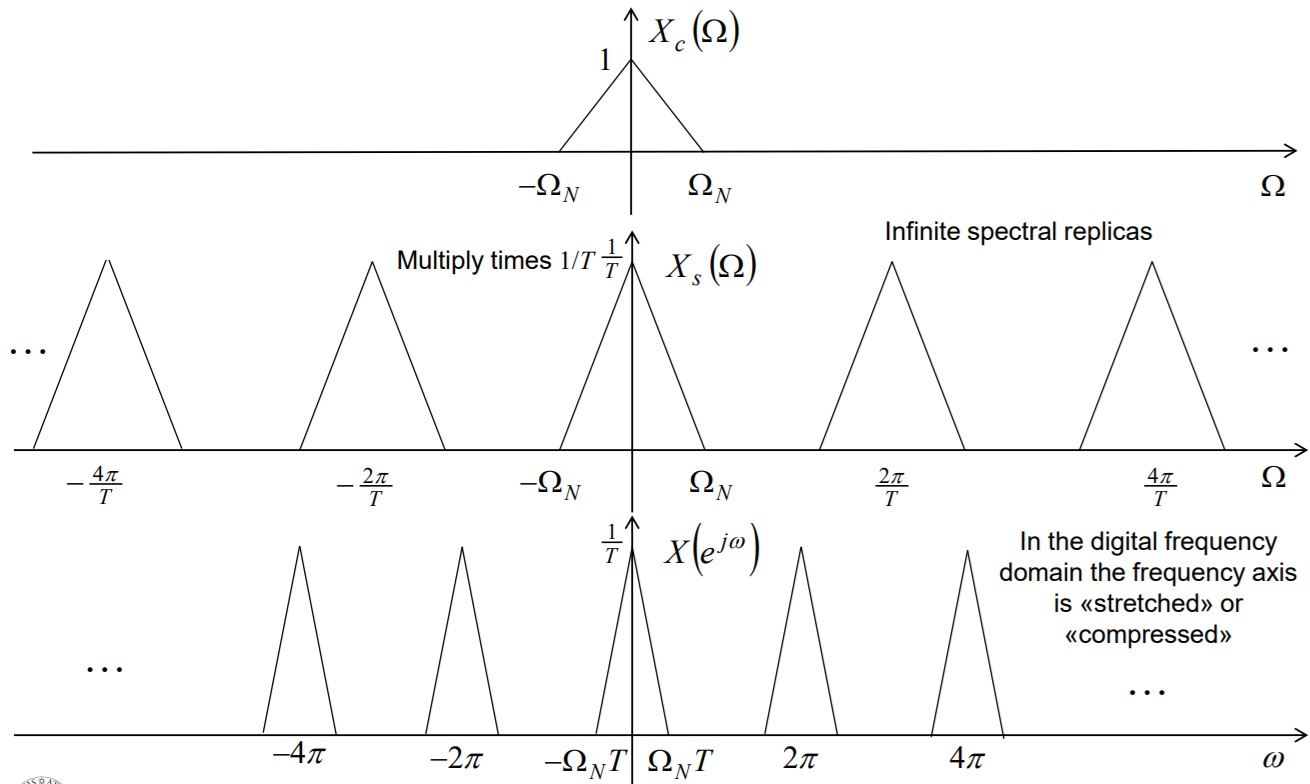
\includegraphics[width=13cm]{replicas}
				\caption{representation of the spectrum of the sampled signal.} \label{fig:conv:replicas}
			\end{figure}
			
			As shown in figure \ref{fig:conv:replicas}, to represent the spectrum $X(e^{j\omega})$ of the discretized signal knowing the original frequency response $X_c(\Omega)$ we have to perform the following steps:
			\begin{enumerate}
				\item build all the spectral replicas at distances $\Omega = \frac{2\pi}{T_s} k$ $\forall k \in \mathds Z$;
				\item multiply all the spectra by a coefficient $1/T_s$;
				\item remap the analog frequency variable $\Omega$ with the digital one $\omega$ using the relation $\omega = \Omega T_s$.
			\end{enumerate}			
		
		\subsection{Nyquist sampling theorem} \label{sec:conv:nyquist}
			
			The introduction of spectral replicas might lead to the problem of \de{aliasing} that happens every time the spectral replicas of the signal (due to the sampling) overlaps in the frequency domain, resulting in a distortion (in that region the frequencies adds up, altering the initial value); this problem arise every time the sampling period is too high (or reciprocally the sampling frequency is too low) respect to the characteristic value of the signal.
			
			The aliasing must always be avoided because the loss of information due to the overlaps of the replicas is irrecoverable and in order to to so it's mandatory to increase the sampling frequency (decrease the sampling period $T_s$) to avoid such overlap. Given $\Omega_n$ as the maximum frequency of the spectrum of the signal that we want to sample, than we have to ensure that
			\begin{equation}
				\Omega_n < \frac \pi {T_s}
			\end{equation}
			This inequality is the base of the \de{Nyquist-Shennon sampling theorem} that states that the maximum frequency of the signal to sample must be less than half of the sampling frequency; knowing that $f_n = \frac{\Omega_n}{2\pi}$ we have in fact that
			\begin{equation} \label{eq:conv:nyquist}
				2\pi f_n < \pi f_s \qquad \Rightarrow \qquad f_n < \frac{f_s}{2}
			\end{equation}
			ensuring so that $\omega_n < \pi$. We refer to the value $f_s/2$ as the \de{Nyquist frequency} and determines the upper bound o the allowable frequency of the input signal in order not to have aliasing. 
			
			The aliasing problem can so be avoided by designing a proper low-pass analog filter before the continuous-to-discrete time converter (in fact in figure \ref{fig:conv:adc} the filter was referred as \textit{anti-aliasing}).		
			
		\subsection{Sample \& hold}
			
			After the time-discretization process has happened, the output passes through a \textbf{Zero-Order Hold} filter that sets as constant the output with a value equal to the input and resets each period $T_s$; this time is in particular chosen in order to allow the ADC block to perform it's conversion operations. Such filter should also avoid the problem of the \textit{shocking} of the transients due to the switch commutations.
			
		
			From a practical point of view the time discretization and the zero-order hold is performed by the \de{sample \& hold amplifier} whose electronic circuit is shown in figure \ref{fig:conv:samplehold}.		
			This kind of circuit implementation resamples a low pass electrical filter; ideally while the sampling signal $v_c$ is set to high, the output $v_y$ is set equal to the input voltage $v_x$ while when $v_c$ is low the exit remains constant (hold operation) due to the ideally constant charge of the capacitor whose also charge time has considered negligible.
			
			Real implementations have to consider both the charge time of the capacitor $C_H$ as well as the fact that the component discharges with time due to parasitic currents; from a design point of view lower capacitances $C_H$ decreases the time required for the charge with the drawback of also increasing the effect of the current leak and so there's always a trade-off between this aspects.
		
			\begin{figure}[bh]
				\centering
				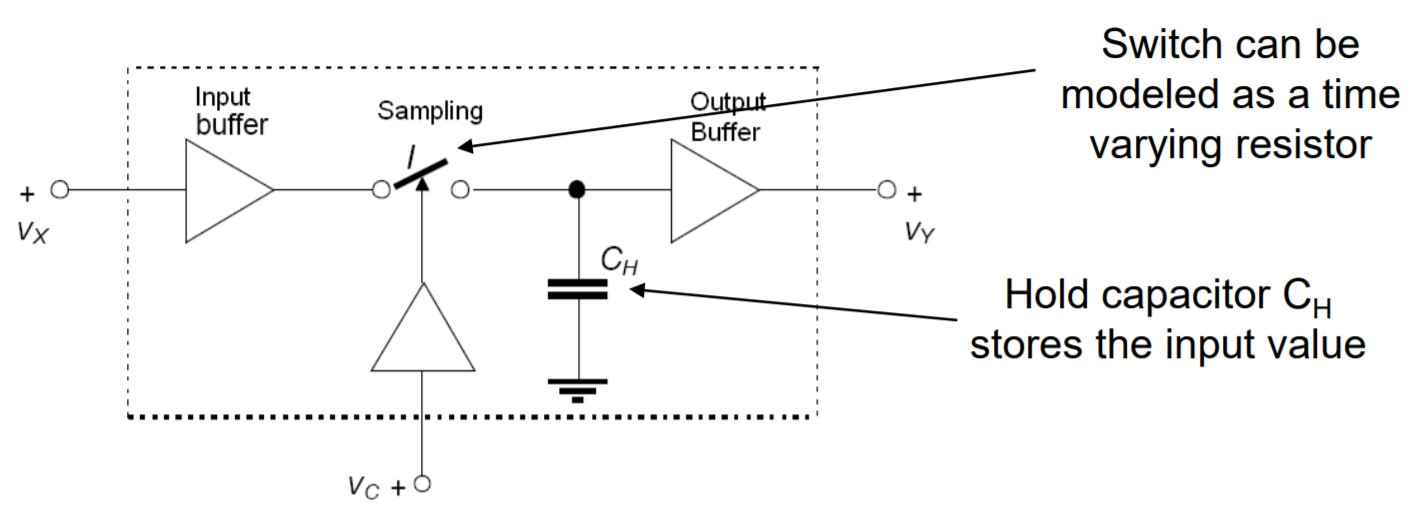
\includegraphics[width = 11cm]{samplehold}
				\caption{possible implementation of an electrical sample \& hold amplifier. }
				\label{fig:conv:samplehold}
			\end{figure}
		\subsection{Quantization and codification}
			
			With a sample \& hold amplifier we have a signal that's constant in the sampling period $T_s$, the next step is to perform the proper analog-to-digital conversion that consists in the operations of \de{quantization} (discretization of the values) and the consequent \de{codification} in binary representation.
			
			\paragraph{Quantization} To quantization action is performed on a pre-defined range (usually on voltages) $[V_{min}, V_{max}]$ that's subdivided into disjoint intervals $I_k = (T_{k-1},T_k]$ where $T_k$ is the $k$-th threshold voltage. Each interval so corresponds to a certain code bin $Q_k$ that's $T_{k}-T_{k-1}$ wide. An ideal analog-to-digital converter has the characteristic that
			\[ Q(x_s) = Q_k \qquad \text{for } T_{k-1} < x_s \leq T_k \]
			By graphically representing this function (figure \ref{fig:conv:quantization}) we can see it \textit{stair-case response} that determines the \textbf{quantization levels} of the quantized.
			
			\begin{SCfigure}[2][bht]
				\centering
				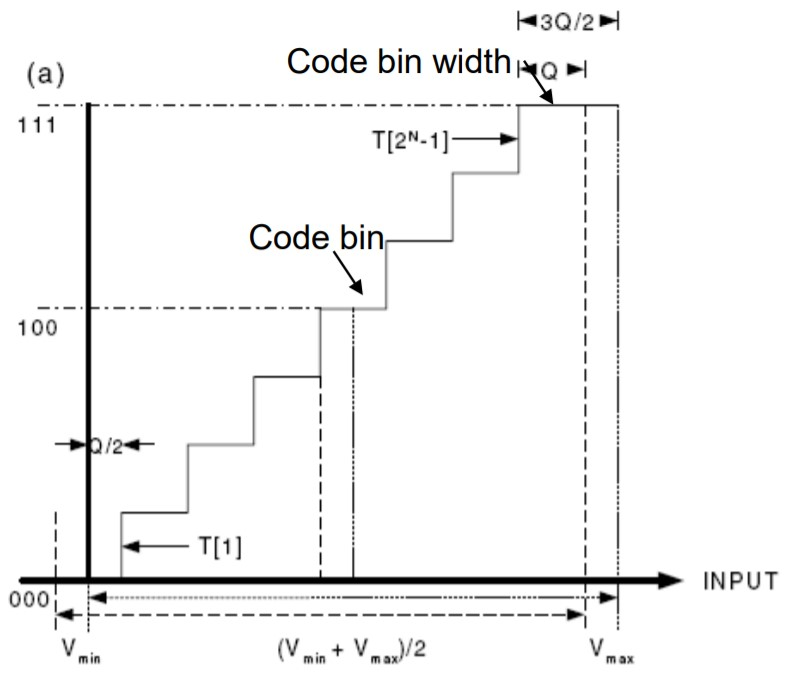
\includegraphics[width=6cm]{quantization}
				\caption{graphical representation of the stair-case function that determine the quantization of a signal.} \label{fig:conv:quantization}
			\end{SCfigure} 
			
			\noindent
			Depending on the possible value of the inputs, ADCs can be classified as
			\begin{itemize}
				\item unipolar if $V_{min} = 0$ and $V_{max} = F_s$;
				\item bipolar if $V_{min} = - F_s$ and $V_{max} = F_s$.
			\end{itemize}
			The number of quantization levels is of course related to the digital implementation of the system: given $b$ the number of bits that the ADC block can output, then the maximum number of allowed bins are $2^b$ with $2^b-1$ quantization thresholds. Assuming to have quantization steps with equal length $\Delta$, then such value can be computed as
			\begin{equation}
				\Delta = \begin{cases}
					\frac{2F_s}{2^b} = \frac{F_s}{2^{b-1}} \qquad & \text{bipolar case} \\
					\frac{F_s}{2^b} \qquad & \text{unipolar case} \\
				\end{cases}
			\end{equation}
			and so increasing the number of bits, the resolution improves exponentially.
			
			\paragraph{Error analysis} As the quantization operation is a non-linear operation a fully analytical model is complex, however if the input signal changes randomly and the difference between two consecutive samples is much larger than the quantization step, the error can be modelled as a realization of additive stochastic processes $e_q(\cdot)$ that can be regarded as
			\begin{itemize}
				\item white and stationary;
				\item uncorrelated to the input signal $x_s$;
				\item with a uniform probability density function.
			\end{itemize} 
			The quantization operation can work with a rounding on the value and the range of uniformity of the PDF is $[-Q/2,Q/2]$ (as shown in figure \ref{fig:conv:quantizationerror}) while if we use a truncation model then the range is shifted becoming $[-Q,0]$. In both case the mean and the variance of the quantization noise is
			\begin{align*}
				\mu_q & = 0 \qquad & \sigma_q^2 & = \frac{Q^2}{12} \qquad && \text{rounding case} \\
				\mu_q & = -\frac Q2 \qquad & \sigma_q^2 & = \frac{Q^2}{12} \qquad && \text{truncation case}
			\end{align*}
		
			\begin{SCfigure}[2][bht]
				\centering
				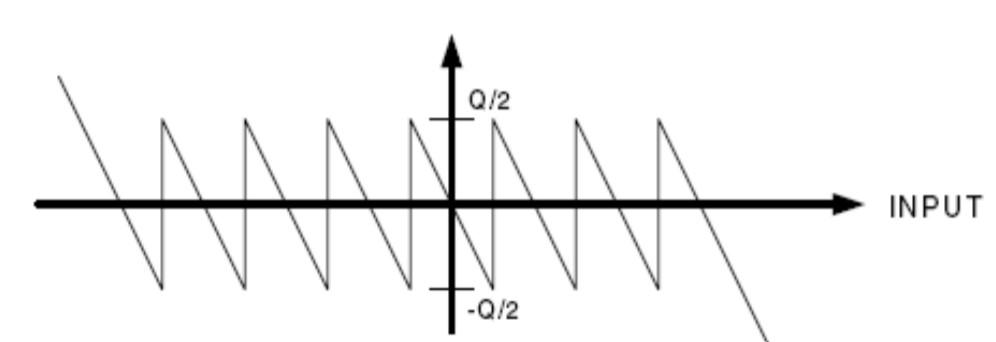
\includegraphics[width=6cm]{quanterror}
				\caption{quantization error due to a rounding quantization.} \label{fig:conv:quantizationerror}
			\end{SCfigure}
			
			\paragraph{Signal-to-noise and quantization ratio} The \textbf{signal-to-noise and quantization ratio} $SQNR$, usually expressed in decibels, is a parameter that allows to compare the variance of the quantization error respect to the one of the original signal:
			\begin{equation}
				SQNR := \frac{\sigma_x^2}{\sigma_q^2}
			\end{equation}
			
			Considering the case of a rounding quantization error, the $SQNR$ parameter in decibel can be expressed as
			\begin{equation}
			\begin{aligned}
				SQNR_{dB} & = 10 \log_{10}\left(\frac{\sigma_x^2}{\sigma_q^2}\right) = 10 \log_{10} \left( \sigma_x^2 \frac 3 {F_s^2} 2^{2b} \right) \\ \Rightarrow \quad SQNR_{dB}  & \approx 6.02b + 20\log_{10}\sigma_x + 20\log_{10} \left( \frac{\sqrt 3}{F_s} \right)
			\end{aligned}
			\end{equation}
			This means that for each bit $b$ added on the quantization level, the potential improvement of the signal-to-noise ratio is of about $6dB$; in general a good rule to design the number of bits to have a low quantization error is
			\begin{equation}
				b = \frac 1 2 \log_2 \left( \frac{\sigma_x^2}{\sigma_q^2} \right)
			\end{equation}
			
			A more accurate description of the analog-to-digital converter performance might take into account other imperfection; considering the original signal $\hat x$
			\[ \hat x(n) = x(n) + e_q(n) + e_\omega(n) \]
			described as the sum of the quantized signal $x$, the quantization error $e_q$and other external noises $e_\omega$ then we can compute the \textbf{signal-to-noise ration} $SNR$ as
			\begin{equation}
				SNR = \log_2 \left( \frac{\sigma_x^2}{\sigma_e^2 + \sigma_\omega^2} \right) < SQNR
			\end{equation}
			This expression has been obtained considering all error as uncorrelated (modelled as white noises) with a more gaussian than normal distribution.
			
			\paragraph{ENOB} In the assumption of having statistically independent noise sources $e_q,e_\omega$, then it's possible to compute the \de{effective number of bits} $ENOB$ as
			\begin{equation}
				ENOB = \frac 1 2 \log_2 \frac{\sigma_x^2}{\sigma_q^2 + \sigma_\omega^2}
			\end{equation}
			Considering so the case of an ADC constructed with a $16bit$ quantization, if the $ENOB$ is lower, like $12bit$ then the last $4$ significant bits are \textit{meaningless} because they are affected by the ADC noises.
						
		\subsection{Technology implementations}
			
			In general analog-to-digital converters are classified in categories depending on their technology implementation that allows to achieve particular performances in terms of number of bits and sampling frequencies. As general behaviour, higher resolution (number of bits) requires lower sample rate while if the number of samples per second required is high, the resolution inevitably drops. As a rule of thumb, decreasing the nominal resolution by a bit determined a double sampling frequency.
			
			\begin{SCfigure}[1][bht]
				\centering
				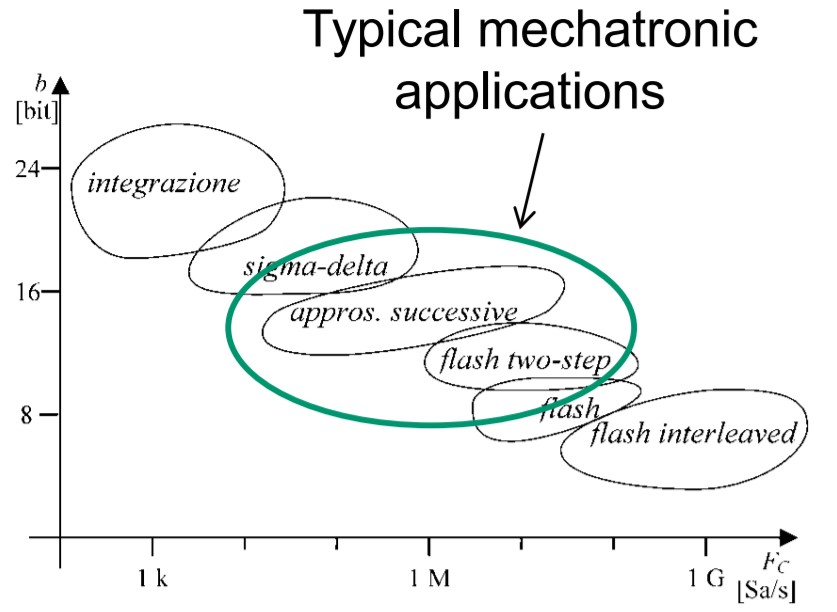
\includegraphics[width=6.5cm]{adc-families}
				\caption{families of analog to digital converters with associated performance as sample per second ($x$ axis) and resolution bits ($y$ axis).}
			\end{SCfigure}
		
			For mechatronics applications usually successive-approximation ADC's (or ones with similar properties) are chosen for having the best trade-off between frequency and resolution.			

\section{Digital-to-analog converter}
	
	A \de{digital-to-analog converter} \textbf{DAC} is a component whose scope is to reconstruct a continuous-time analog signal from a discrete-time digital value.
	
	Given the discrete-time input sequence $y(n)$ that has to be transformed in the continuous-time signal $y_c(\cdot)$, the reconstruction can happens simply considering an ideal \textbf{low-pass reconstruction filter} with gain $T_s$ and cut-off frequency of $\pi/T_s$. From a spectral point of view the obtained result is
	\begin{equation}
		Y_c(\Omega) = T_s \, Y\big(e^{j\Omega T_s}\big) \qquad \textrm{for } |\Omega| \leq \frac \pi {T_s}
	\end{equation}
	Intuitively the gain of $T_s$ is due to the fact that, in the analog-to-digital conversion, the spectra was attenuated by a multiplicative factor $1/T_s$ and so the low-pass reconstructor filter must \textit{compensate} for such error; the filter should also be low-pass in order to avoid the propagation of the spectral replicas of the sampled signal.
	
	\begin{figure}[bht]
		\centering 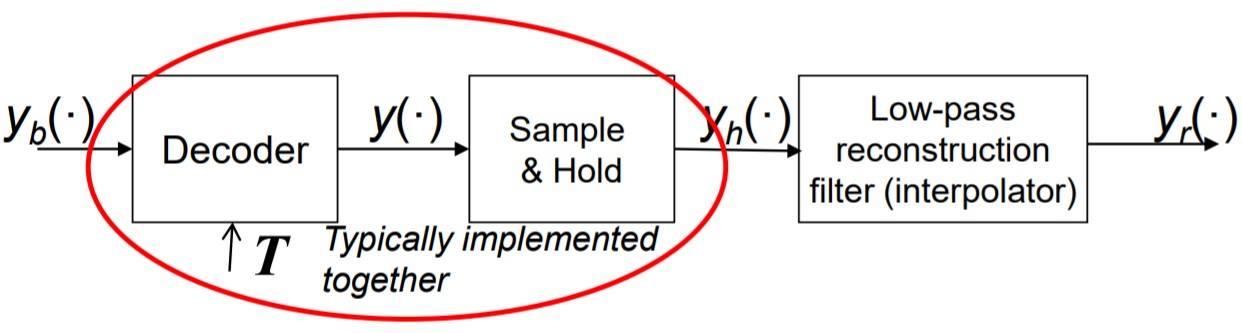
\includegraphics[width=10cm]{DAC-scheme}
		\caption{schematic  representation of the steps/components used to perform a digital-to-analog conversion.} \label{fig:conv:DACscheme}
	\end{figure}
	
	\paragraph{Real DAC considerations} Considering a real implementation of a digital-to-analog converter, as shown in figure \ref{fig:conv:DACscheme}, 3 main steps must be performed:
	\begin{enumerate}
		\item decodification of the digital value into (generally) an analog voltage; such operation is performed by a \textbf{decoder};
		\item after the decoding, a \textbf{sample \& hold} operation must take place for a sampling period $T_s$: this allows to re-introduce the concept of \textit{time} that in the digital domain was lost. Usually this component is automatically embedded in the decoder implementation;
		\item lastly a \textbf{low-pass reconstructor filter}, also called \textbf{\textit{interpolator}}, is used to avoid replicas and to \textit{smoothen} the output.
	\end{enumerate}
	
	Considering the schematic representation of figure \ref{fig:conv:DACscheme}, the signal $y_h(t)$ resulting from the sample \& hold operation is a staircase function that can be described as
	\begin{align*}
		y_h(t) & = \infsum n y(n) \rect_{T_s} \left( t - \frac{T_s}2 - nT_s \right) = \infsum n y_c (nT_s) \rect_{T_s}\left( t - \frac {T_s} 2 - nT_s \right) \\
		& = y_c(t) \left[ \rect_{T_s} \left( t - \frac{T_s}{2} \right) * \infsum n \delta(t-nT_s) \right]
	\end{align*}
	Using the properties of the \ctft (in particular the convolution and the windowing theorem), then the spectra of the signal $y_h$ can be regarded as
	\begin{equation}
	\begin{aligned}
		Y_h(\Omega) & = Y_c(\Omega) * \left[ T_s \sin\left(\frac{\Omega T_s}{2}\right) e^{-j\Omega \frac{T_s}{2}}  \frac 1 {T_s} \infsum k \delta\left( \Omega - \frac{2\pi k}{T_s} \right) \right] \\
		& = Y(\Omega) T_s \sinc \left(\frac{\Omega T_s}{2}\right) e^{-j\Omega \frac{T_s}2}
	\end{aligned}
	\end{equation}
	From this expression we can see that the spectrum resulting from the zero-order-hold is a modified (by a $\sinc$ function) frequency response from $Y(\Omega)$ generated by the decoder. The ideal implementation of the reconstructor filter $\hat H_r$ is so to compensate the non-ideal behaviours introduced by the zero-order-hold and so
	\begin{equation}
		\hat H_r = \begin{cases}
			\frac{T_s}{H_h(\Omega)} \qquad & |\Omega|\leq\frac{\pi}{T_s} \\ 0 & \textrm{otherwise}
		\end{cases}
	\end{equation}
	
	
	
\section{Multi-rate signal processing}
	
	Until now we consider conversions with a defined sampling frequency $f_s = 1 / T_s$, however sometimes it might be necessary to increase or decrease such value to perform better analysis; in particular frequency should be increase if the processor cannot \textit{keep up in speed} with the real-time processing, while increasing speed might be good to have a better read-out in the time domain.
	
	In general we refer as \de{multi-rate signal processing} the operation that allows, starting from a fixed sampling frequency $f_s$, to decrease (\textbf{undersampling} case) or increase (\textbf{upsampling}) the number of samples per second.

	\subsection{Undersampling}
		
		The \de{undersampling} operation, referred also as \textbf{decimation}, is an operation that decreases the sampling rate by a so called \textbf{decimation factor} $M$ (that's an integer value). The \de{compressor} (figure \ref{fig:conv:compressor}) is the \textit{block} that so performs the undersampling operation by selecting $1$ over $M$ samples. Mathematically, given the \textit{full} input discrete-time sequence $x(n)$, the compressor determines a new sequence
		\begin{equation}
			x_d(n) = x(nM) \hspace{2cm} M \in \mathds N
		\end{equation}
		
		\begin{SCfigure}[2][bht]
			\centering 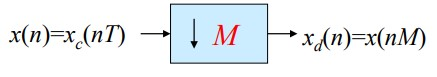
\includegraphics[width=6cm]{compressor}
			\caption{compressor performing an undersampling with decimation factor $M$.} \label{fig:conv:compressor}
		\end{SCfigure}
		
		Determined $T_s' = M T_s$ the new \textit{decimated} sampling period, we can describe the impact of this operation by analysing the spectral changes in the output of the system:
		\begin{equation}
		\begin{aligned}
			X_d\big(e^{j\Omega T_s'}\big) & = \frac 1{MT_s} \infsum k X_c\left( \Omega - \frac{2\pi k}{MT_s} \right)  = \frac 1{T_s'} \infsum k X_c\left( \Omega - \frac{2\pi k}{T_s'} \right)  \\
			X_d(e^{j\omega}) & = \frac 1 {T_s'} \infsum k X_c\left( \frac{\omega}{T_s'} - \frac{2\pi k}{T_s'}\right)
		\end{aligned}
		\end{equation}
		From this expression we can see that the main draw-back of undersampling is that it narrows the distance of the spectral replicas that in the discrete frequencies domain $\omega$ correspond to a shrink of a factor $1/M$, as shown in figure \ref{fig:conv:undersamplingresults}. The loss of information due to a lower sampling frequency is caused by the aliasing, and so to avoid such problem we have to be sure that
		\[ X_c\big( e^{j\omega} \big) = 0 \hspace{2cm} \textrm{for } |\omega|\geq \frac \pi M \]
 		This assertion can be ensured by pre-processing the input sequence $x_c(n)$ with a low-pass filter with unitary gain and cut-off frequency of $\pi/M$.
 		
 		\begin{SCfigure}[2][bht]
 			\centering 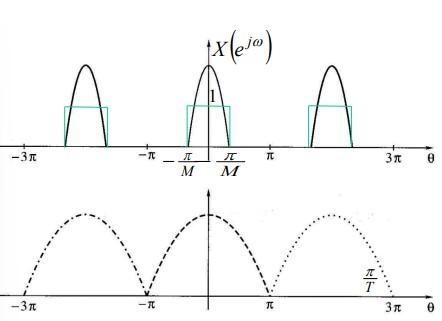
\includegraphics[width=6cm]{downsampling}
 			\caption{original spectra $X_c(e^{j\omega})$ and it modification after a decimation with $M=2$.} \label{fig:conv:undersamplingresults}
 		\end{SCfigure}	
	
	\subsection{Upsampling}
		
		The goal of \de{upsampling}, also referred as \textbf{interpolation}, is increasing the sampling frequency by decreasing the sampling period by a \textbf{interpolation factor} $L$:
		\[ T_s' = \frac{T_s}{L} \hspace{2cm} L \in \mathds N \]
		
		\begin{SCfigure}[2][bt]
			\centering 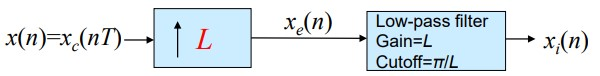
\includegraphics[width=0.5\linewidth]{upsampling}
			\caption{interpolation scheme with an expander and a interpolator block.}
			\label{fig:conv:upsamplingscheme}
		\end{SCfigure}
	
		This operation, performed by the \de{expander} (figure \ref{fig:conv:upsamplingscheme}), add new samples in the sequence by adding $L-1$ zeros after each sample, determining the expanded sequence defined as
		\begin{equation}
		x_e(n) = \begin{cases}
			x(n/L) \qquad & n = 0,\pm L, \pm 2 L,\pm 3L \dots \\
			0 & \textrm{otherwise}
		\end{cases}
		\end{equation}		
		
		Upon this sequence we can calculate it's \dtft resulting in 
		\begin{equation}
		\begin{aligned}
			X_e\big(e^{j\omega}\big) & = \infsum n x_e(n) e^{-j\omega n} = \infsum k x(k) e^{-j\omega kL} = X\big(e^{j\omega'}\big) \\
			& = \frac 1{T_s} \infsum k X_c\left( \frac{\omega'}{T_s} - \frac{2\pi k}{T_s} \right) = \frac 1{LT_s'} \infsum k X_c\left( \frac{\omega}{T_s'} - \frac{2\pi k}{LT_s'} \right)
		\end{aligned}
		\end{equation}
		where $\omega' = \omega L$. From a graphical point of view (figure \ref{fig:conv:upsampling}) this expression shrinks the original replicas by a factor $L$ (multiplication by $1/L$) and adds new replicas every $T_s/L$; the magnitude has also been reduced by a factor $L$. In order so to remove the new images created and \textit{resize} the spectrum a discrete-time interpolating low-pass filter with gain $L$ and cut-off frequency $\pi/L$ is required.
		
		\begin{SCfigure}[2][bht]
			\centering 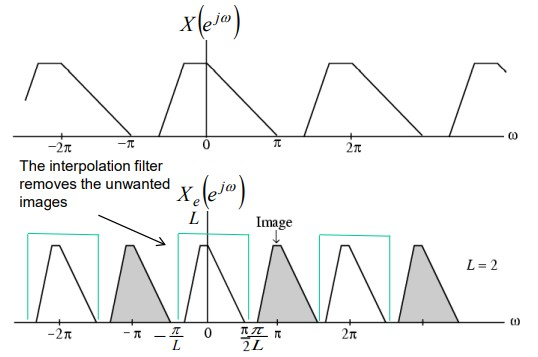
\includegraphics[width=0.5\linewidth]{upsampling-graph}
			\caption{original spectrum due to the sampling of a signal (upper) and upsampled spectrum (bottom) of the same signal with a value $L=2$.}
			\label{fig:conv:upsampling}
		\end{SCfigure}
		
		
		
		
		
		
		
		
	
	
	
	
	
	
	
	
	
	
	
	
	
	
	
	
	
	
	
	
	
	
	
	
	
	
	
	
	
	
	
	